\documentclass[a4paper, titlepage]{article}

% For equations
\usepackage{amsmath}

% For including figures
\usepackage{graphicx}

% For typesetting matlab
\usepackage{listings}
\usepackage{color} %red, green, blue, yellow, cyan, magenta, black, white
\definecolor{mygreen}{RGB}{28,172,0} % color values Red, Green, Blue
\definecolor{mylilas}{RGB}{170,55,241}

\lstset{language=Matlab,%
    %basicstyle=\color{red},
    breaklines=true,%
    morekeywords={matlab2tikz},
    keywordstyle=\color{blue},%
    morekeywords=[2]{1}, keywordstyle=[2]{\color{black}},
    identifierstyle=\color{black},%
    stringstyle=\color{mylilas},
    commentstyle=\color{mygreen},%
    showstringspaces=false,%without this there will be a symbol in the places where there is a space
    numbers=left,%
    numberstyle={\tiny \color{black}},% size of the numbers
    numbersep=9pt, % this defines how far the numbers are from the text
    emph=[1]{for,end,break},emphstyle=[1]\color{red}, %some words to emphasise
    %emph=[2]{word1,word2}, emphstyle=[2]{style},    
}


\title{Assignment 1\\
System description and analysis\\
\large EEA004}
\author{Dan Thilderkvist, Philip Gutierrez}

\begin{document}

\maketitle

\section{Background/Introduction}
This assignment study an air handling system with a heater and a humidifier, figure \ref{fig:airSystem}.
The system allow control of two variables, temperature $y_1$ and humidity $y_2$.
This can be done through the flow of of a heater $u_1$ and the flow of a humidifier $u_2$.

\begin{figure}
\center
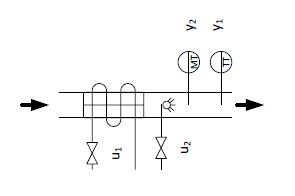
\includegraphics[scale=1]{../figures/heaterHumidifier.png}
\caption{Air management system with heater $u_1$, humidifier $u_2$, thermometer $y_1$ and hygrometer $y_2$.}
\label{fig:airSystem}
\end{figure}

Although the system is not linear, it is assumed linear within a small region of operation.
With this in mind both the heater and the humidifier can be modeled as first order systems, [\ref{equ:firstOrder}].

\begin{equation}
G(s) = \frac{K}{\tau s + 1}
\label{equ:firstOrder}
\end{equation}

The time constant $\tau$ has been given for the heater $\tau_1=50$ and for the humidifier $\tau_2=10$ in the assignment.
The static gain $K$ will have to be calculated for each system.
For that purpose the assignment include two enthalpy–entropy charts, one for each system.
There is also information provided how the system reacts to a step input of $u_1 = 1$ or $u_2 = 2$.
The heater open fully $u_1 = 1$ will increase incoming air of $10^\circ C, 40\% \: RH$ by $15^\circ C$ and the humidifier open fully will increase incoming air of $20^\circ C, 10\% \: RH$ by $70\% \: RH$.

\subsection{Theory}
A linear system can be represented on state space form.
The general form of a state space formulation is as follows:

\begin{equation}
\begin{split}
\dot{x} &= Ax + Bu \\
y &= Cx + Du
\end{split}
\end{equation}


The final value theorem is something that is often used for system identification.
It can especially come in handy when a system is exited by a step input and the steady state output after a long time can be measured.
The final value theorem states:

\begin{equation}
\lim_{t \to \infty} f(t) = \lim_{s \to 0} sF(s)
\label{equ:finalTheorem}
\end{equation}

Observability of a system loosely indicate if the system states can be reconstructed from the output, if a system is observable the observer poles can be placed arbitrarily.
The observability matrix is defined as such:

\begin{equation}
\mathcal{O}(A,C) = 
\begin{pmatrix}
C \\ CA \\ \vdots \\ CA^{n-1}
\end{pmatrix}
\end{equation}

If the observability matrix $\mathcal{O}$ has full rank (independent rows/columns) the system is observable.
In a similar fashion, controllability loosely indicate if all states of a system can be controlled by the input, if a system is controllable the poles of a state feedback controller can be arbitrarily chosen.
The Controllability matrix is defined as such:

\begin{equation}
\mathcal{S}(A,B) = 
\begin{pmatrix}
B & AB & \cdots & A^{n-1}C
\end{pmatrix}
\end{equation}

If the controllability matrix $\mathcal{S}$ has full rank (independent rows/columns) the system is controllable.

\section{Method}
This section will describe the work flow of identifying the air handling system, doing basic analysis on the identified system and in the end designing a controller for for it.

\subsection{System identification}
The air handling system described in the introduction is one of multiple input multiple output (MIMO).
Such a system will have a transfer function matrix $\boldsymbol{G}(s)$ from input to output. In this particular case it will be a $2x2$ matrix because of the two input $u_1, u_2$ and the two output $y_1, y_2$.
The system can be written as such:

\begin{equation}
\begin{split}
\boldsymbol{Y}(s) &= \boldsymbol{G}(s)\boldsymbol{U}(s) \leftrightarrow \\
\begin{pmatrix}
Y_1 \\ Y_2
\end{pmatrix}
&=
\begin{pmatrix}
G_{11}(s) & G_{12}(s) \\ G_{21}(s) & G_{22}(s)
\end{pmatrix}
\begin{pmatrix}
U_1(s) \\ U_2(s)
\end{pmatrix}
\end{split}
\end{equation}

Both heater and humidifier is apporximated by first order systems [\ref{equ:firstOrder}].
Hence the transfer function elements can be written:

\begin{equation}
G_{ij}(s) = \frac{K_{ij}}{\tau_{ij} s + 1}
\end{equation}

Where $\tau_{11} = \tau_{12} = \tau_1 = 50$ and $\tau_{21} = \tau_{22} = \tau_2 = 10$ are given in the introduction.

In order to find $K_{ij}$ the final value theorem [\ref{equ:finalTheorem}] can be applied along with the steady state information from the introduction.

\begin{equation}
\lim_{t \to \infty} y_{1}(t) = 
\lim_{s \to 0} sY_{1}(s) = 
\lim_{s \to 0} s(G_{11}(s)U_{1} + G_{12}(s)U_{2})
\end{equation}

\begin{equation}
G_{u_1y_1}(0) = K = 15degree
\end{equation}

\begin{equation}
G_{u_1y_2}(0) = K = -25\% 
\end{equation}

\begin{equation}
G_{u_2y_1}(0) = K = -10degree 
\end{equation}

\begin{equation}
G_{u_2y_2}(0) = K = 70\% 
\end{equation}

\section{Results}

\subsection{Question 1}

\subsection{Question 2}

\begin{equation}
\begin{split}
\dot{x} &= 
\begin{pmatrix}
-0.02 & 0 \\ 0 & -0.1
\end{pmatrix}x
+
\begin{pmatrix}
0.3 & -0.5 \\ -0.25 & 1.75
\end{pmatrix}u \\
y &= 
\begin{pmatrix}
1 & 0 \\ 0 & 4
\end{pmatrix}x
\end{split}
\end{equation}

\subsection{Question 3}

\subsection{Question 4}

\subsection{Question 5}

\begin{equation}
U(s) = -L_y(s)Y(s) + L_r(s)R(s) 
\end{equation}



\section{Conclusion/Discussion}


\section{Example code}

\includegraphics[scale=0.8]{../code/figures/exampleFigure.png}

\lstinputlisting{../code/exampleCode.m}

\end{document}